\documentclass[10pt,a4paper]{exam}
\usepackage[utf8]{inputenc}
\usepackage{amsmath}
\usepackage{amsfonts}
\usepackage{bbm}
\usepackage{commath}
\usepackage{amssymb}
\usepackage{booktabs}
\usepackage{blkarray}
\usepackage{systeme}
\usepackage{graphicx}
\usepackage[left=.75in,right=.75in,top=.75in,bottom=.75in]{geometry}

\usepackage{tikz}
\usetikzlibrary{chains}
\printanswers


\author{Ryan Honea}
\title{Time Series Analysis Homework 3}
\begin{document}
\begin{center}
Time Series Homework 3\\
Ryan Honea
\end{center}
\begin{questions}
\question Find ACF and ACVF of the following processes. Also use R to plot them.
\begin{parts}
\part $X_t = e_t + \frac{5}{2}e_{t-1} - \frac{3}{2}e_{t-2}$ where $e_t \sim WN(0,1)$

\begin{solution}
\begin{align*}
E[X_t]			&= E\left[e_t + \frac{5}{2}e_{t-1} - \frac{3}{2}e_{t-2}\right]\\
					&= E[e_t] + \frac{5}{2}E[e_{t-1}] - \frac{3}{2}E[e_{t-2}]\\
					&= 0\\
\gamma(t, t+h)		&= Cov\left(e_t + \frac{5}{2}e_{t-1} - \frac{3}{2}e_{t-2}, e_{t+h} + \frac{5}{2}e_{t+h-1} - \frac{3}{2}e_{t+h-2}\right)\\
							&= Cov(e_t, e_{t+h}) + \frac{5}{2}Cov(e_t, e_{t+h-1}) - \frac{3}{2}Cov(e_t, e_{t+h-2})\\
							&+ \frac{5}{2}Cov(e_{t-1}, e_{t+h}) + \frac{25}{4}Cov(e_{t-1}, e_{t+h-1}) - \frac{15}{4}Cov(e_{t-1}, e_{t+h-2})\\
							&- \frac{3}{2}Cov(e_{t-2}, e_{t+h}) - \frac{15}{4}Cov(e_{t-2}, e_{t+h-1}) + \frac{9}{4}Cov(e_{t-2}, e_{t+h-2})\\
\implies \gamma(0)		&= 1 + \frac{25}{4} + \frac{9}{4}\\
						&= \frac{19}{2}\\
\implies \gamma(\pm1)		&= -\frac{5}{4}\\
\implies \gamma(\pm2)		&= -\frac{3}{2}
\end{align*}

From the above, we have therefore

\begin{align*}
\gamma(h) 		&= 	\begin{cases}
									\frac{19}{2}, & h = 0\\
									-\frac{5}{4}, & h = \pm 1\\
									-\frac{3}{2}, & h = \pm 2\\
									0, & \text{o/w}
								\end{cases}\\
\rho(h)				&= 	\begin{cases}
									1, & h = 0\\
									-\frac{5}{38},	& h = \pm 1\\
									-\frac{3}{19},		& h = \pm 2\\
									0, & \text{o/w}\\
								\end{cases}
\end{align*}
\begin{center}
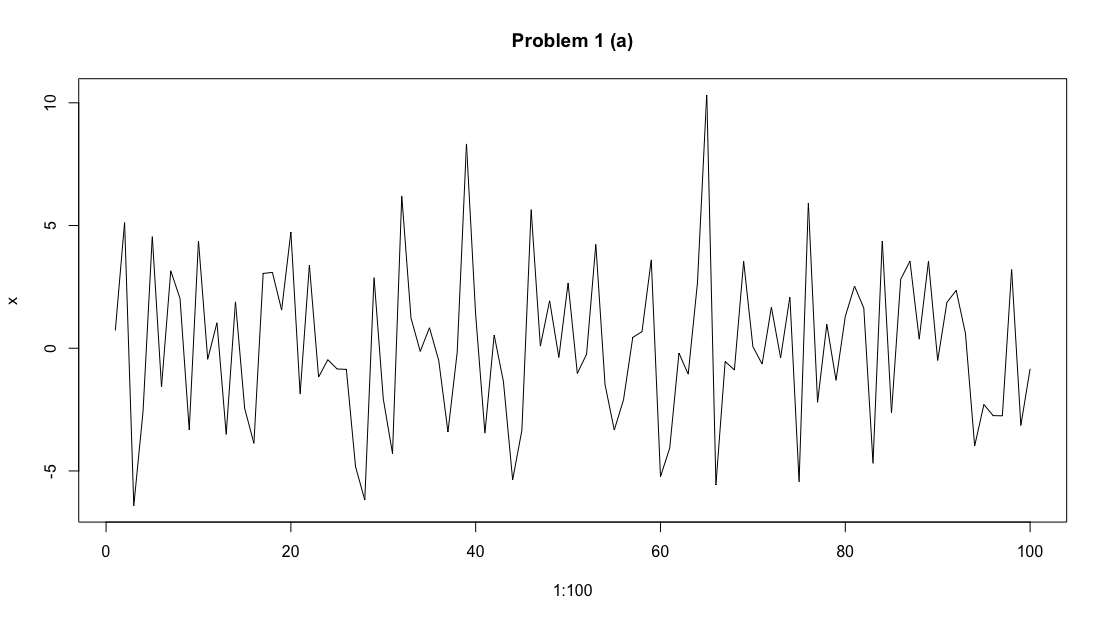
\includegraphics[width=.9\linewidth]{P1A}
\end{center}
\end{solution}

\pagebreak

\part $X_t = e_t - \frac{1}{6}e_{t-1} - \frac{1}{6}e_{t-2}$ where $e_t \sim WN(0,9)$

\begin{solution}
\begin{align*}
E[X_t]		&= E\left[e_t - \frac{1}{6}e_{t-1} - \frac{1}{6}e_{t-2}\right]\\
				&= E[e_t] - \frac{1}{6}E[e_{t-1}] - \frac{1}{6}E[e_{t-2}]\\
				&= 0\\
\gamma(t, t+h)	&= Cov\left(e_t - \frac{1}{6}e_{t-1} - \frac{1}{6}e_{t-2}, e_{t+h} - \frac{1}{6}e_{t+h-1} - \frac{1}{6}e_{t+h-2} \right)\\
						&= Cov(e_t, e_{t+h}) - \frac{1}{6}Cov(e_t, e_{t+h-1}) - \frac{1}{6}Cov(e_t, e_{t+h-2})\\
						& -\frac{1}{6}Cov(e_{t-1}, e_{t+h}) +\frac{1}{36}Cov(e_{t-1}, e_{t+h-1}) +\frac{1}{36}Cov(e_{t-1}, e_{t+h-2})\\
						& -\frac{1}{6}Cov(e_{t-2}, e_{t+h}) +\frac{1}{36}Cov(e_{t-2}, e_{t+h-1}) +\frac{1}{36}Cov(e_{t-2}, e_{t+h-2})\\
\implies \gamma(0)	&= 9 + \frac{9}{36} + \frac{9}{36}\\
								&= \frac{19}{2}\\
\implies \gamma(\pm 1)	&= -\frac{5}{4}\\
\implies \gamma(\pm 2)	&= -\frac{3}{2}
\end{align*}

From the above, we have therefore

\begin{align*}
\gamma(h) 		&= 	\begin{cases}
									\frac{19}{2}, & h = 0\\
									-\frac{5}{4}, & h = \pm 1\\
									-\frac{3}{2}, & h = \pm 2\\
									0, & \text{o/w}
								\end{cases}\\
\rho(h)				&= 	\begin{cases}
									1, & h = 0\\
									-\frac{5}{38},	& h = \pm 1\\
									-\frac{3}{19},		& h = \pm 2\\
									0, & \text{o/w}\\
								\end{cases}
\end{align*}
\begin{center}
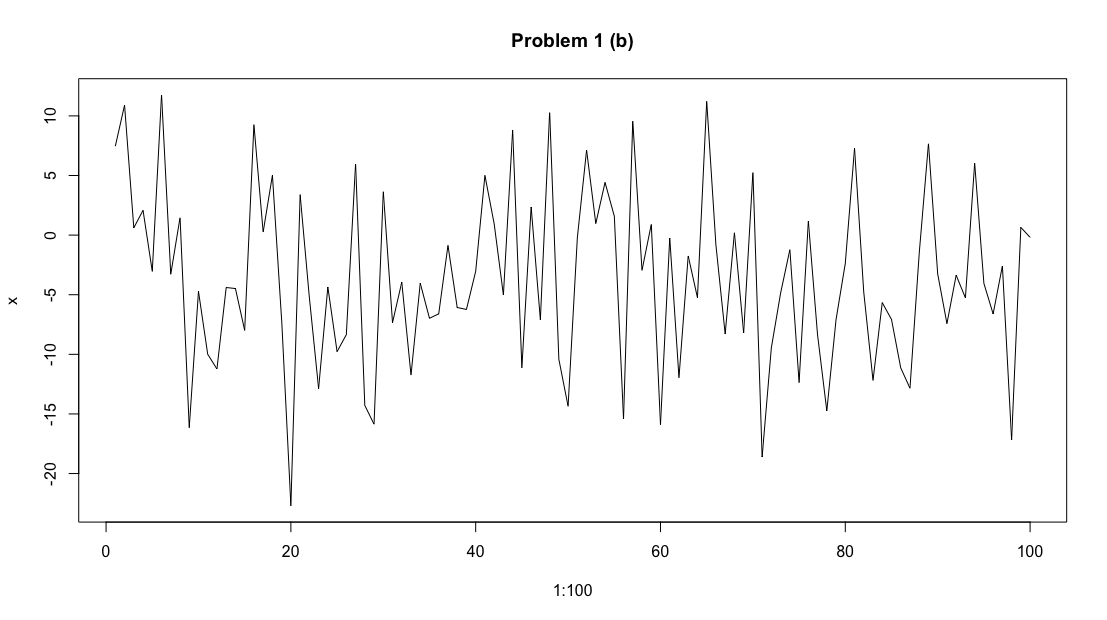
\includegraphics[width=\linewidth]{P1B}
\end{center}
\end{solution}

\part Which of these models in $a$ and $b$ are (i) invertible, (ii) causal and (iii) stationary?
\begin{solution}
\textbf{Part (a):}\\
We have $X_t = e_t\left(1 + \frac{5}{2}B - \frac{3}{2}B^2\right)$. The roots of this are $-\frac{1}{3}$ and $2$, so it is not invertible. It is, however, causal, as $X_t$ can be represented as the sum of the current and past $e_t$s. we also know that any $MA(q)$ process is causal. It is also shown above that this process satisfies the conditions of stationarity.

\textbf{Part (b):}\\
We have $X_t = e_t - \frac{1}{6}e_{t-1} - \frac{1}{6}e_{t-2}$ or $X_t = e_t\left(1 - \frac{1}{6}B - \frac{1}{6}B^2\right)$ which has roots $2$ and $-3$, so it is invertible. For the reasons before, it is also causal. It is also shown above that this process satisfies the conditions of stationarity.
\end{solution}
\end{parts}

\question For each of the following ARMA models, find the roots of the AR and MA polynomials, identify the values of $p$ and $q$ for which they are $ARMA(p,q)$ (be careful of parameter redundancy), determine whether they are causal, and determine whether they are invertible. In each case, $e_t \sim WN(0,1)$.

\begin{parts}
\part $X_t + 0.81X_{t-2} = e_t + \frac{1}{3}e_{t-1}$
\begin{solution}
Using the back-shift operator, we have 
$$X_t(1 + .81B^2) = e_t\left(1 + \frac{1}{3}B\right)$$
which is hypothetically $ARMA(2,1)$.

The roots of the left side are $\pm \frac{10}{9}i$ and so the process is causal. The roots of the right side are $-3$ and so the process is invertible.

As the polynomials share no common factors, this process is indeed $ARMA(p,q)$.
\end{solution}

\part $X_t - X_{t-1} = e_t - 0.5e_{t-1} - 0.5e_{t-2}$
\begin{solution}
Using the back-shift operator, we have
$$X_t(1 - B) = e_t(1 - 0.5B - 0.5B^2)$$

The factors on the left are $1$ and the factors on the right are $-2$ and $1$. Therefore we have
\begin{align*}
X_t(1 - B) 		&= e_t(B+2)(1 - B)\\
			X_t	&= e_t(B+2)
\end{align*}

so this reduces to an $ARMA(0,1)$ process which is just an $MA(1)$ process with root $-2$ so it is invertible and causal.
\end{solution}

\part $X_t - 3X_{t-1} = e_t + 2e_{t-1} - 8e_{t-2}$
\begin{solution}
Using the back-shift operator, we have
$$X_t(1 - 3B) = e_t\left(1 +2B - 8B^2\right)$$
This is hypothetically $ARMA(1,2)$.

On the left side, the roots are $\frac{1}{3}$ and so it is not causal. On the right side, the roots are $\frac{-1}{4}$ and $\frac{1}{2}$ so it is not invertible.

As there are no common factors in the left and right polynomials, then it is $ARMA(1,2)$.
\end{solution}
\pagebreak

\part $X_t - 2X_{t-1} + 2X_{t-2} = e_t - \frac{8}{9}e_{t-1}$
\begin{solution}
Using the back-shift operator, we have
$$X_t(1 - 2B + 2B^2) = e_t\left(1 - \frac{8}{9}B\right)$$
This is hypothetically $ARMA(2,1)$.

On the left side, the roots are $\frac{1}{2} \pm \frac{i}{2}$ so it is not causal. On the right side, the root is $\frac{9}{8}$ so it is invertible.

As the are no common factors in the left and right polynomials, then it is $ARMA(2,1)$.
\end{solution}

\part $X_t - 4X_{t-2} = e_t - e_{t-1} + 0.5e_{t-2}$
\begin{solution}
Using the back-shift operator, we have
$$X_t(1 - 4B^2) = e_t(1 - B + 0.5B^2)$$
This is hypothetically $ARMA(2,2)$.

On the left side, the roots are $\pm \frac{1}{2}$ so it is not causal. On the right side, the roots are $1 \pm i$ so it is invertible.

As the are no common factors in the left and right polynomials, then it is $ARMA(2,2)$.
\end{solution}

\part $X_t - \frac{9}{4}X_{t-1} - \frac{9}{4}X_{t-2} = e_t$
\begin{solution}
Using the back-shift operator, we have
$$X_t\left(1 - \frac{9}{4}B - \frac{9}{4}B^2\right) = e_t$$
which is an $ARMA(2,0)$ process which is just $AR(2)$.

The roots of the $AR$ process are $\frac{1}{3}$ and $-\frac{4}{3}$ so the process is not causal.
\end{solution}
\end{parts}
\pagebreak

\question For those processes in the previous problem that are causal, plot the ACF and PACF function. Also, compute the first 10 coefficients in the causal representation of those models.

\begin{parts}
\part  $X_t + 0.81X_{t-2} = e_t + \frac{1}{3}e_{t-1}$
\begin{solution}
\begin{center}
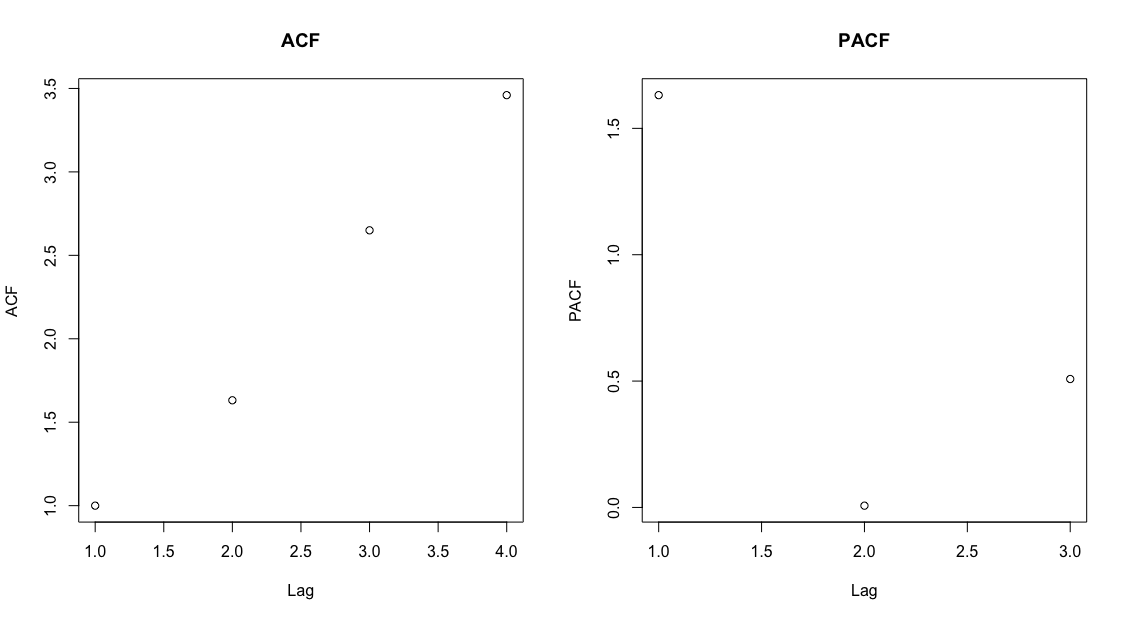
\includegraphics[width=.8\linewidth]{P3A}
\end{center}
Using the formula
$$\psi_j = \theta_j + \sum_{k=1}^2 \phi_k \psi_{j-k}$$
and then the R code derived from it

\begin{verbatim}
phi <- rep(0,10); phi[2] <- .81
theta <- rep(0,10); theta[1] <- 1/3
psi <- rep(1, 11); psi[2] <- theta[1]
for (i in 3:11) {
  psi[i] <- theta[i-1] + phi[2]*psi[i-2]
}
\end{verbatim}

the coefficients are 
\begin{align*}
\psi_1 &= 1/3 & \psi_2 &= .81\\
\psi_3 &= .27 & \psi _4 &\approx .66\\
\psi_5 &\approx .22 & \psi_6 &\approx .53\\
\psi_7 &\approx .18 & \psi_8 &\approx .43\\
\psi_9 &\approx .14 & \psi_{10} &\approx .35
\end{align*}
\end{solution}

\pagebreak
\part $X_t - X_{t-1} = e_t - 0.5e_{t-1} - 0.5e_{t-2}$
\begin{solution}
When utilizing the armaACF function, the results are singular so an approximate plot it made below.
\begin{verbatim}
library(forecast)
e <- rnorm(500,0,1)
x <- c()
x[1] <- 0
x[2] <- 0
for (i in 3:500) {
  x[i] <- e[i] - 0.5*e[i-1] - 0.5*e[i-2] + x[i-1]
}
plot(1:500, x, type = "l", main = "Problem 3 (b)")
par(mfrow = c(1,2))
Acf(x)
Pacf(x)
\end{verbatim}
we get
\begin{center}
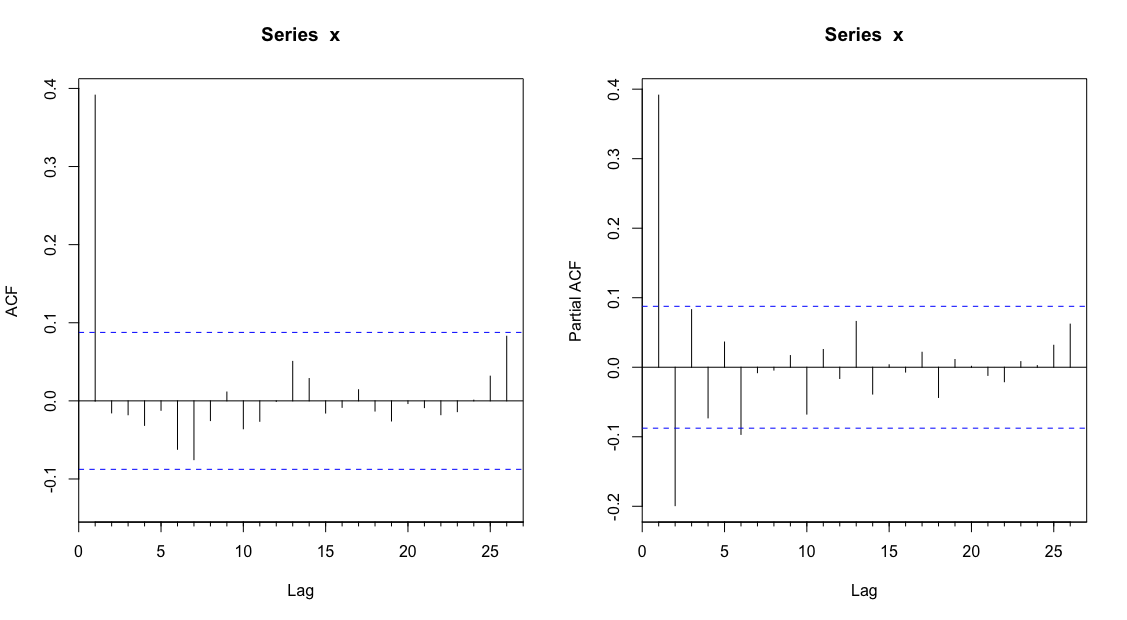
\includegraphics[width=.8\linewidth]{P3B}
\end{center}

In 2(b), we showed that this process is an MA process which is already in it's causal representation, so the coefficients are $\psi_0 = 2.0$ and $\psi_1 = 1$ and 0 elsewhere.

\end{solution}
\end{parts}
\pagebreak

\question Show that for a MA(1) process $|\rho(1)| \leq 1/2$.
\begin{solution}
An $MA(1)$ process is defined as
$$X_t = e_t + \theta e_{t-1} \quad \text{with} \quad \rho(1) = \gamma(1)/\gamma(0)$$
That is, we have
\begin{align*}
\rho(1)			&= \gamma(1)/\gamma(0)\\
					&= \frac{\sigma^2_e \theta}{\sigma^2_e (1 + \theta^2)}\\
					&= \frac{\theta}{1 + \theta^2}\\
\frac{\dif \rho(1)}{\dif \theta}	
					&= \frac{1-\theta^2}{\left(1 + \theta^2\right)^2}
\end{align*}
Setting the above derivative gives $\rho(1)$ maximized for $\theta = 1$ and minimized for $\theta = -1$. So we have
\begin{align*}
\min \rho(1)	&= \frac{-1}{1 + (-1)^2}			& \max \rho(1)	&= \frac{1}{1 + 1^2}\\
					&= \frac{-1}{2}						&						&	\frac{1}{2}
\end{align*}

Therefore, the range of $\rho(1)$ is $\left[-\frac{1}{2},\frac{1}{2}\right]$ and so $|\rho(1)| \leq \frac{1}{2}$.
\end{solution}

\question Show that for a MA(1) process, $X_t = e_t + \theta e_{t-1}$, partial auto correlation at lag 2 is:
$\phi_{22} = \dfrac{-\theta^2}{1 + \theta^2 + \theta^4}$, where $e_t \sim WN(0,1)$, and $|\theta| < 1$

\begin{solution}
Utilizing the Durbin Levinson algorithm from the text
$$\phi_{nn} = \left[\gamma(n) - \sum_{j=1}^{n-1} \phi_{n-1,j}\gamma(n-j)\right]v_{n-1}^{-1}$$
we have
\begin{align*}
\phi_{22} 		&= \left[\gamma(2) - \phi_{11}\gamma(1)\right]v_1^{-1}\\
					&= \frac{-\phi_{11}\gamma(1)}{\gamma(0)\left[1 - \phi_{11}\right]} = \frac{-\phi_{11}^2}{\left(1 - \phi_{11}\right)^2}\\
					&= \frac{-\left(\frac{\theta}{1+\theta^2}\right)^2}{1 - \left(\frac{\theta}{1+\theta^2}\right)^2}\\
					&= \frac{-\theta^2}{(1+\theta^2)^2 - \theta}\\
					&= \frac{-\theta^2}{1 + \theta^2 + \theta^4}
\end{align*}
\end{solution}
\pagebreak

\question Let $X_t = e_t + \theta e_{t-1}$ be a MA(1) process, with $e_t \sim WN(0, \sigma_e^2)$. Find another MA(1) process with the same ACVF as $X_t$.

\begin{solution}
The autocovariance function for this process is
$$\gamma(h) = \begin{cases}
\sigma^2_e (1 + \theta^2),			& h = 0\\
\sigma^2_e \theta				,		& h = \pm 1\\
0,												& o/w
\end{cases}$$

Now, let $X_t^* = -e_t -\theta e_{t-1}$ be a MA(1) process.

\begin{align*}
\gamma(t, t+h)		&= Cov\left(-e_t - \theta e_{t-1}, -e_{t+h} - \theta e_{t+h-1}\right)\\
							&= Var(e_t) + \theta^2Var(e_t) & \text{for }h = 0\\
							&= \sigma^2_e (1 + \theta^2) & \text{for }h = 0\\
							&= \theta Var(e_{t+h}) & \text{for }h = \pm 1\\
							&= \theta \sigma^2_e & \text{for }h = \pm 1\\
							&= 0& \text{for }h = 0
\end{align*}
which is an equal ACVF as $X_t$.
\end{solution}


















































\question Consider the process $X_t = \phi X_{t-1} + e_t$, where $e_t \sim WN(0, \sigma^2)$. Assume that the process starts at $t = 0$ and $X_0 = e_0$. Prove that (i) $Var(X_t) = \dfrac{\sigma^2}{1 - \phi^2}[1 - \phi^{2(t+1)}]$ and (ii) $Cov(X_t, X_{t+h}) = \phi^h Var(X_t)$. Is the process stationary as $t \to \infty$?

\begin{solution}
\\\textbf{Part (i):}\\
\begin{align*}
Var(X_t) 	&= Var(\phi X_{t-1} + e_t)\\
				&= \phi^2Var(X_{t-1}) + \sigma^2\\
				&= \phi^2\left(\phi^2\left(Var(X_{t-2}\right) + \sigma^2\right) + \sigma^2\\
				&= \sigma^2 \sum_{i=0}^t \phi^{2i} = \sigma^2 \sum_{i=0}^t \left(\phi^2\right)^i\\
				&= \sigma^2 \left[1 + \sum_{i=1}^t \left(\phi^2\right)^i \right]\\
				&= \sigma^2 \left[1 + \frac{\phi^2 - \phi^{2t+2}}{1 - \phi^2}\right]\\
				&= \sigma^2 \left[\frac{1 - \phi^2 + \phi^2 - \phi^{2t+2}}{1 - \phi^2}\right]\\
				&= \frac{\sigma^2}{1 - \phi^2}\left[1 - \phi^{2(t+1)}\right]
\end{align*}
\end{solution}
\pagebreak
\begin{solution}
\\\textbf{Part (ii):}\\
\begin{align*}
Cov(X_t, X_{t+h})		&= Cov\left(\sum_{i=0}^t \phi^{t-i}e_i, \sum_{i=0}^{t+h} \phi^{t+h-i}e_i\right)\\
								&= \sum_{i=0}^t \sum_{j=0}^{t+h} Cov(\phi^{t-i}e_i, \phi^{t+h-j}e_j)\\
								&= \sum_{i=0}^t \phi^{2t - 2i + h} Cov(e_i, e_i) \quad \quad \text{as }Cov(e_i, e_j) = 0\text{ when }i\neq j\\
								&= \phi^h \sum_{i=0}^t \phi^{2(t-i)} Var(e_i) = \phi^h \sigma^2 \sum_{i=0}^t \left(\phi^2\right)^{t-i}\\
								&= \phi^h \sigma^2 \sum_{i=0}^t \left(\phi^2\right)^i\\
								&= \phi^h Var(X_t)\\
\end{align*}

\textbf{Stationarity:}
In regards to expectation, the expectation will remain a sum of an infinite number of white noise processes which would still be 0. For the variance, we have
\begin{align*}
\lim_{t \to \infty} Var(X_t)		&=  \lim_{t \to \infty} \frac{\sigma^2}{1 - \phi^2}\left[1 - \phi^{2(t+1)}\right]\\
											&=  \frac{\sigma^2}{1 - \phi^2}\lim_{t \to \infty}\left[1 - \phi^{2(t+1)}\right]\\
\lim_{t \to \infty}\left[1 - \phi^{2(t+1)}\right]			&= \begin{cases}
																				1,	& \text{when }|\phi| < 1\\
																				-\infty,	& \text{when } |\phi| > 1\\
																			\end{cases}\\
\end{align*}
From here, we know that $\{X_t\}$ is not stationary when $|\phi| > 1$. As covariance is a constant times the variance, the same condition holds. 

Therefore, $\{X_t\}$ is stationary as $t \to \infty$ only when $|\phi| < 1$
\end{solution}
\pagebreak

































\question Consider an $ARMA(p,q)$ process $\{X_t\}$, satisfying $\phi(B)X_t = \theta(B)e_t$, with $e_t \sim WN(0, \sigma_e^2)$ and ACVF $\gamma_x(h)$. Define a new process $Y_t = X_t + \omega_t$, with $\omega_t \sim WN(0, \sigma_w^2)$. Assume $\mathbb{E}[e_tw_t] = 0$ for all $t$ and $s$. Prove that $Y_t$ is a stationary process and compute its ACVF in terms of $\sigma^2_w$ and $\gamma_x(h)$. Also show that $\phi(B)Y_t$ is a $MA(r)$ process where $r = \max(p,q)$.

\begin{solution}
Firstly, if we let $X_t$ be it's causal representation, (assuming it is causal), then $Y_t$ is the sum of $e_t$s and $\omega_t$ and therefore it's expectation is 0. In regards to the ACVF, we have

\begin{align*}
\gamma(t, t+h)				&= Cov(Y_t, Y_{t+h})\\
									&= Cov(X_t + \omega_t, X_{t+h} + \omega_{t+h})\\
									&= Cov(X_t, X_{t+h}) + Cov(X_t, \omega_{t+h}) + Cov(\omega_t, X_{t+h}) + Cov(\omega_t, \omega_{t+h})\\
									&= Cov(X_t, X_{t+h}) + Cov(\omega_t, \omega_{t+h})\\
									&= \gamma_x(h) + Cov(\omega_t, \omega_{t+h})\\
									&= 	\begin{cases}
												\gamma_x(0) + \sigma_w^2,	& h = 0\\
												\gamma_x(h),	& o/w
											\end{cases}\\
\end{align*}

So it is stationary. Now, let
$$X_t = \theta(B)\phi^{-1}(B)e_t$$

And so this implies
$$\phi(B) Y(t) = \phi(B)\psi(B)\phi^{-1}(B)e_t + \phi(B)\omega_t = \theta(B)e_t + \phi(B) \omega_t$$

As this is the sum of $q$ $e_t$ and $p$ $\omega_t$ variables, then it is necessary to have $r$ back-shift operators in total, so it is an $MA(r)$ process.
\end{solution}








\pagebreak





















\question Consider an AR(2) model $X_t = \phi_1 X_{t-1} + \phi_2 X_{t-2} + e_t$. Show that the process is stationary iff all the following conditions are met:
\begin{parts}
\part $\phi_2 < 1 + \phi_1$
\part $\phi_1 < 1 + \phi_2$
\part $\phi_2 > -1$
\end{parts}

\begin{solution}
An AR model is stationary iff it is causal. For an AR model to be causal, its roots must be outside the unit circle. If we express $X_t$ with the backshift operator, we have
$$X_t(1- \phi_1 B - \phi_2 B^2) = e_t$$
And so we can find the conditions with
\begin{align*}
\frac{\phi_1 + \sqrt{\phi_1^2 + 4\phi_2}}{2} &< -1			& \frac{\phi_1 - \sqrt{\phi_1^2 + 4\phi_2}}{2} &> 1\\
\sqrt{\phi_1^2 + 4\phi_2} 		&< -2 - \phi_1						& -\sqrt{\phi_1^2 + 4\phi_2} &> 2 - \phi_1\\
\phi_1^2 + 4\phi_2 		&< \phi_1^2 + 4\phi_1 + 4					& \phi_1^2 + 4\phi_2 &< \phi_1^2 - 4\phi_1 + 4\\
4\phi_2 &< 4\phi_1 + 4					& 4\phi_2 &< -4\phi_1 + 4\\
\phi_2 &< 1 + \phi_1					& \phi_2 &< 1 - \phi_1
\end{align*}
So, we have the first two conditions. Note that these don't match the first two conditions given in the homework problem, but after graphing the three conditions, I'm not sure it makes sense to use the conditions given.

In the above, we considered the real roots, and so now in considering the imaginary roots we have
$$B_1 = \frac{\phi_1 + i\sqrt{\phi_1^2 + 4\phi_2}}{2} \quad \quad B_2 = \frac{\phi_1 - i\sqrt{\phi_1^2 + 4\phi_2}}{2}$$
which are conjugate pairs. We need $|B_1B_2| < 1$ for stationarity and we find that to be

$$B_1B_2 = \frac{\phi_1^2 - \phi_1^2 - 4\phi_2}{4} = -\phi_2$$

Therefore, we must also have $|-\phi_2| < 1$ which implies $\phi_2 > -1$.

\end{solution}
\end{questions}
\end{document}